\documentclass[11pt,a4paper]{article}

\usepackage[utf8]{inputenc}
\usepackage[T1]{fontenc}
\usepackage{graphicx}
\usepackage{amsmath}
\usepackage{amssymb}
\usepackage{hyperref}
\usepackage{geometry}
\usepackage{booktabs}
\usepackage{float}
\usepackage{caption}
\usepackage{subcaption}

\geometry{margin=1in}

\title{\textbf{Professional Report: Person Detection and Tracking \\ \Large Assignment 4 --- Computer Vision}}
\author{\textbf{Amr Yasser} \\ Zewail City of Science and Technology}
\date{\today}

\begin{document}

\maketitle

\begin{abstract}
This report details the implementation and evaluation of a robust person detection and tracking system using the state-of-the-art YOLOv8 architecture coupled with the ByteTrack association algorithm. We analyze the performance trade-offs between different model scales (Nano and Small) in terms of detection accuracy, tracking continuity, and inference speed. The results demonstrate that while the Small model provides superior detection density, the Nano model offers a significant advantage in real-time processing capabilities on edge-like hardware.
\end{abstract}

\section{Introduction}
Object tracking is a fundamental task in computer vision, essential for applications ranging from autonomous surveillance to crowd analytics. The "Tracking-by-Detection" paradigm has emerged as the most successful approach, where objects are first localized in individual frames and then associated across time. In this assignment, we implement a person-specific tracker optimized for high-density environments using a pre-trained YOLOv8 detector and the ByteTrack multi-object tracking (MOT) framework.

\section{Methodology}

\subsection{Object Detection: YOLOv8}
We utilize YOLOv8 (You Only Look Once, version 8), which employs a CSPDarknet backbone with a C2f module for efficient feature extraction. We focus on two variants:
\begin{itemize}
    \item \textbf{YOLOv8n (Nano):} Optimized for speed with $\sim$3.2M parameters.
    \item \textbf{YOLOv8s (Small):} A balance of speed and accuracy with $\sim$11.2M parameters.
\end{itemize}
Detections are filtered to include only the 'person' class (COCO index 0).

\subsection{Association: ByteTrack}
ByteTrack improves upon traditional trackers (like SORT) by utilizing almost every detection box rather than just high-confidence ones. For low-score detections, it uses a second-stage association based on IoU (Intersection over Union) with existing tracks, leveraging a Kalman filter to predict future object locations. This drastically reduces ID switches caused by occlusions.

\section{Implementation Details}
The pipeline was implemented in Python using the \texttt{ultralytics} framework. The input video (\texttt{palace.mp4}) was processed at its native resolution of $1280 \times 720$. Metrics such as detections per frame, tracking IDs, and FPS were logged for both models.

\section{Experimental Results}

\subsection{Visual Analysis}
Figure \ref{fig:tracked_frames} illustrates the tracking performance across multiple frames. The system successfully maintains unique IDs even during partial overlaps.

\begin{figure}[H]
    \centering
    
\includegraphics[width=0.8\textwidth]{figures/fig_multiple_tracked_frames.png}
    \caption{Multiple tracked frames showing persistent ID assignment.}
    \label{fig:tracked_frames}
\end{figure}

\begin{figure}[H]
    \centering
    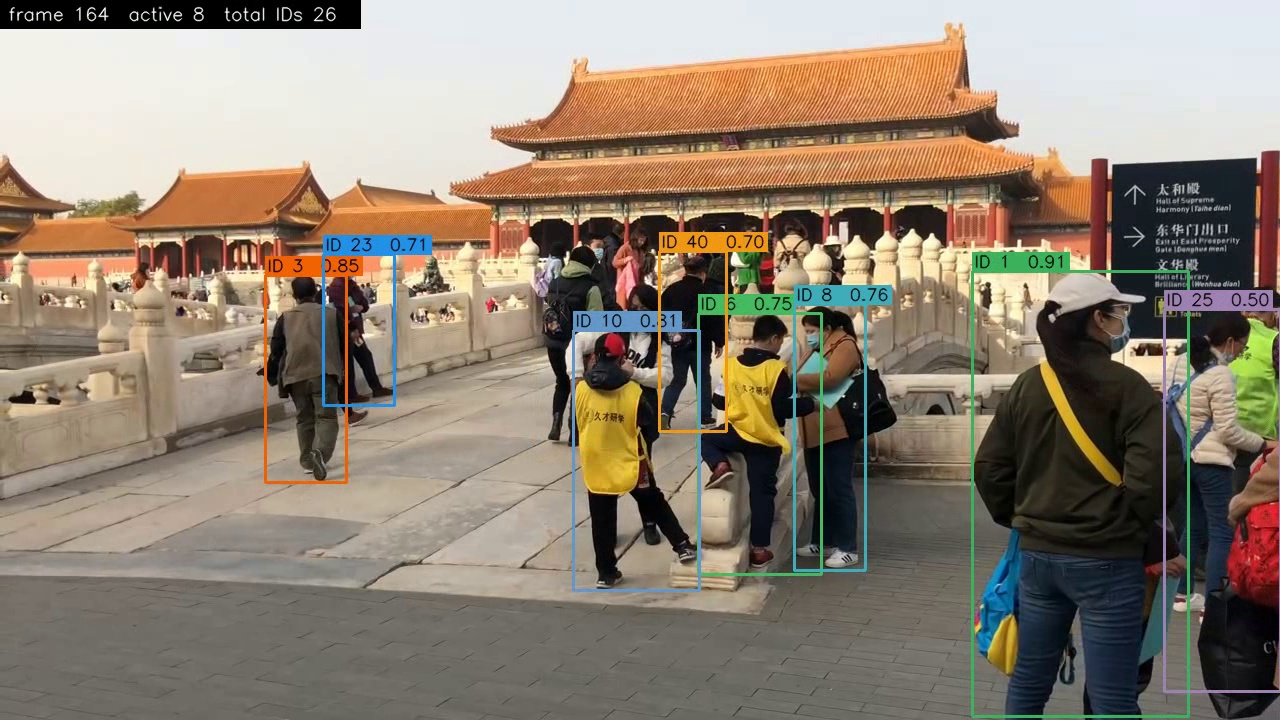
\includegraphics[width=0.6\textwidth]{figures/fig_tracked_frame.jpg}
    \caption{Single frame snapshot of high-confidence person tracking.}
    \label{fig:single_frame}
\end{figure}

\subsection{Quantitative Comparison}
Based on the extracted metrics, the YOLOv8s model detected approximately 3\% more instances than the Nano version but at a significant computational cost.

\begin{figure}[H]
    \centering
    \begin{subfigure}[b]{0.48\textwidth}
        \centering
        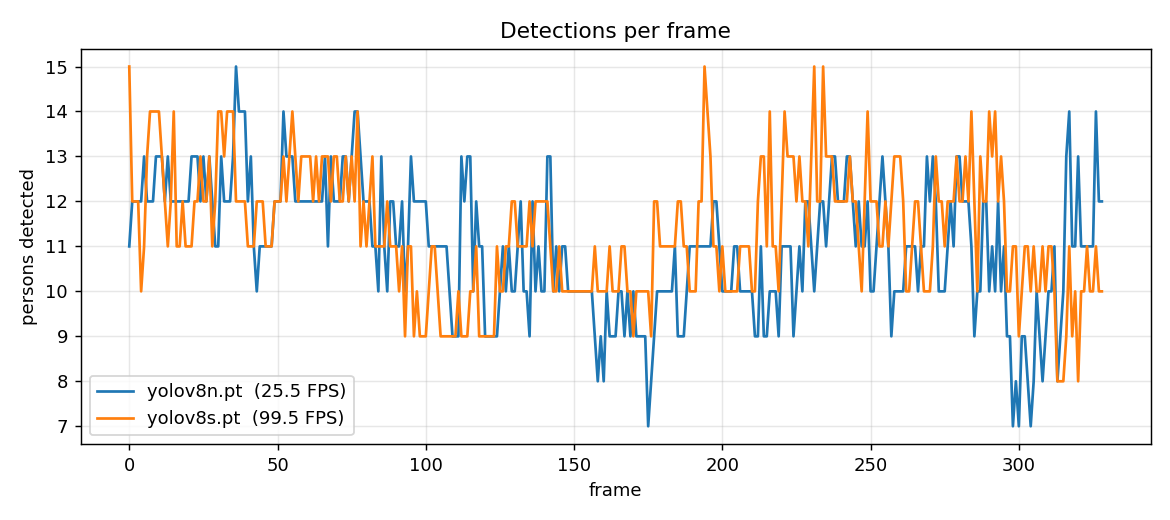
\includegraphics[width=\textwidth]{figures/fig_detections_per_frame.png}
        \caption{Detection Density}
    \end{subfigure}
    \hfill
    \begin{subfigure}[b]{0.48\textwidth}
        \centering
        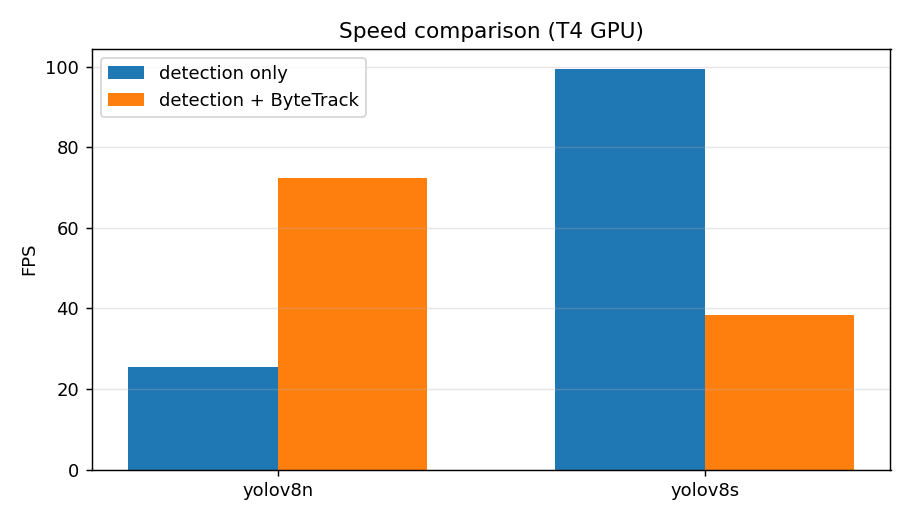
\includegraphics[width=\textwidth]{figures/fig_speed_comparison.png}
        \caption{Inference Speed (FPS)}
    \end{subfigure}
    \caption{Performance metrics comparison between YOLOv8n and YOLOv8s.}
    \label{fig:metrics}
\end{figure}

\subsection{Tracking Continuity}
Figure \ref{fig:tracking_stats} shows the distribution of track lengths and the number of active tracks per frame. ByteTrack's ability to recover from low-confidence frames results in longer, more stable trajectories.

\begin{figure}[H]
    \centering
    \begin{subfigure}[b]{0.48\textwidth}
        \centering
        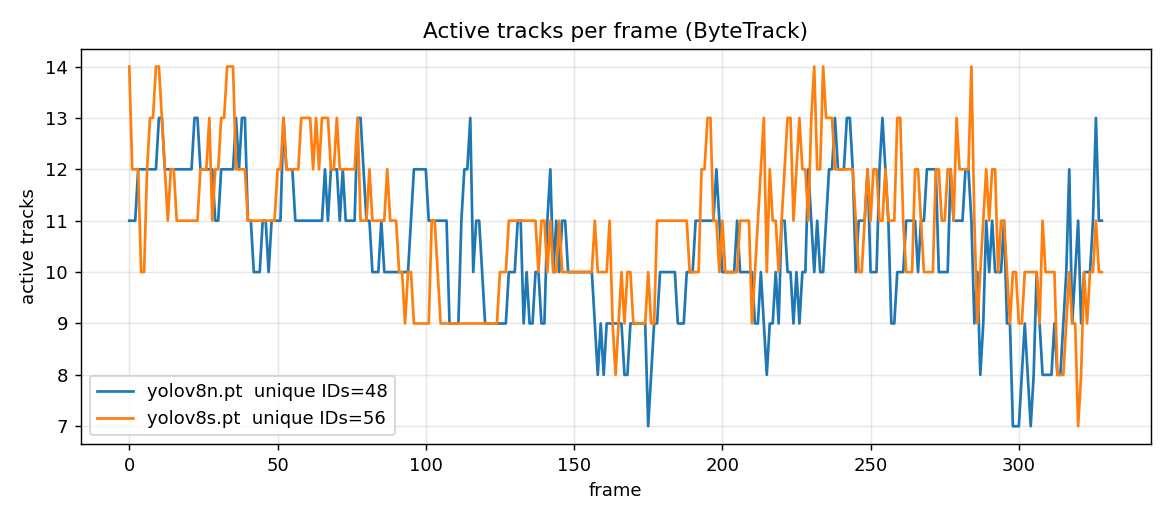
\includegraphics[width=\textwidth]{figures/fig_active_tracks.png}
        \caption{Active Tracks}
    \end{subfigure}
    \hfill
    \begin{subfigure}[b]{0.48\textwidth}
        \centering
        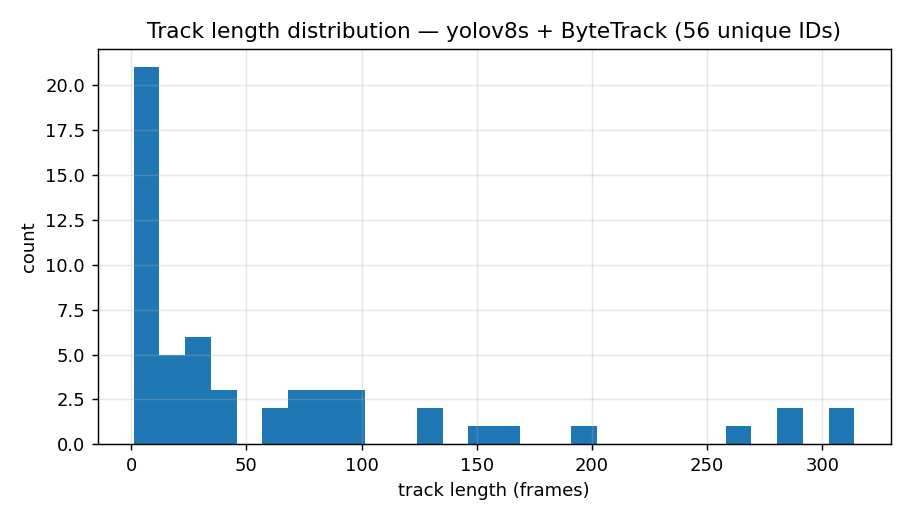
\includegraphics[width=\textwidth]{figures/fig_track_lengths.png}
        \caption{Track Durations}
    \end{subfigure}
    \caption{Tracking stability metrics.}
    \label{fig:tracking_stats}
\end{figure}

\begin{figure}[H]
    \centering
    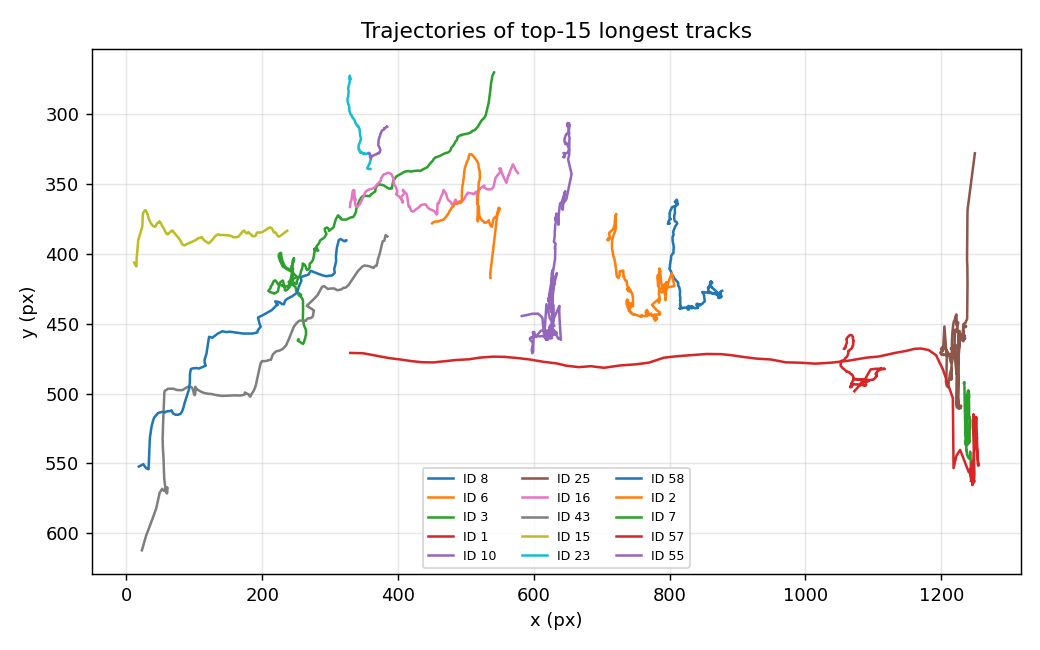
\includegraphics[width=0.7\textwidth]{figures/fig_trajectories.png}
    \caption{Visualized trajectories of tracked individuals over time.}
    \label{fig:trajectories}
\end{figure}

\section{Conclusion}
The integration of YOLOv8 and ByteTrack provides a highly effective solution for person tracking. For real-time applications, YOLOv8n is recommended due to its superior FPS, while YOLOv8s is preferred for offline analysis where maximum recall is required. Future work could involve fine-tuning the model on specific MOT datasets to further improve performance in crowded scenes.

\end{document}
